% CELLAIR Status Update — Follow-up to Elevator Pitch
% Compile with: pdflatex main.tex (twice for references)
\documentclass[aspectratio=169,11pt]{beamer}

% ============================================================
% Theme: Clean, minimal — matches 01_elevator_pitch
% ============================================================
\usetheme{default}
\usecolortheme{default}

% Colors — University of Salzburg corporate design
\definecolor{unisalz}{RGB}{17, 87, 64}          % Grün PANTONE 343 C
\definecolor{unisalzgray}{RGB}{156, 156, 156}   % Grau PANTONE Cool Grey 9
\definecolor{unisalzlight}{RGB}{214, 232, 226}  % light green tint
\definecolor{alertred}{RGB}{180, 40, 40}        % alert/warning
\definecolor{donegreen}{RGB}{40, 130, 70}       % completed
\definecolor{progressamber}{RGB}{200, 130, 30}  % in progress

\setbeamercolor{structure}{fg=unisalz}
\setbeamercolor{frametitle}{fg=unisalz, bg=white}
\setbeamercolor{title}{fg=unisalz}
\setbeamercolor{subtitle}{fg=unisalzgray}
\setbeamercolor{author}{fg=unisalzgray}
\setbeamercolor{date}{fg=unisalzgray}
\setbeamercolor{institute}{fg=unisalzgray}
\setbeamercolor{normal text}{fg=black, bg=white}
\setbeamercolor{block title}{fg=white, bg=unisalz}
\setbeamercolor{block body}{bg=unisalzlight}
\setbeamercolor{alerted text}{fg=alertred}
\setbeamercolor{headlinecolor}{fg=unisalzgray, bg=white}
\setbeamercolor{footlinecolor}{fg=unisalzgray, bg=white}

% Remove navigation symbols
\setbeamertemplate{navigation symbols}{}

% ============================================================
% Header
% ============================================================
\setbeamertemplate{headline}{%
  \begin{beamercolorbox}[wd=\paperwidth, ht=0.55cm, dp=0.2cm]{headlinecolor}%
    \hspace{0.7em}%
    \raisebox{-0.1cm}{
\includegraphics[height=0.38cm]{img/Siegel-300x300-corpgrey.png}}%
    \hspace{0.25em}%
    {\small\color{unisalzgray} universit\"{a}t}%
    {\small\color{unisalz}\bfseries salzburg}%
    \hfill%
    {\small\color{unisalz}\bfseries ag}%
    {\small\color{unisalzgray} lepperdinger}%
    \hspace{0.6em}\phantom{x}%
  \end{beamercolorbox}%
  \begin{beamercolorbox}[wd=\paperwidth, ht=0.4pt]{structure}%
  \end{beamercolorbox}%
}

% ============================================================
% Footer
% ============================================================
\setbeamertemplate{footline}{%
  \begin{beamercolorbox}[wd=\paperwidth, ht=0.4pt]{structure}%
  \end{beamercolorbox}%
  \begin{beamercolorbox}[wd=\paperwidth, ht=0.45cm, dp=0.2cm]{footlinecolor}%
    \hspace{0.6em}%
    {\footnotesize\color{unisalzgray}%
      \insertframenumber\,/\,\inserttotalframenumber}%
    \hfill%
    {\footnotesize\color{unisalzgray}\usebeamertemplate{frame subtitle}}%
    \hspace{0.6em}%
  \end{beamercolorbox}%
}

% ============================================================
% Packages
% ============================================================
\usepackage[T1]{fontenc}
\usepackage{lmodern}
\usepackage{graphicx}
\usepackage{booktabs}
\usepackage{amsmath}
\usepackage[version=4]{mhchem}
\usepackage{siunitx}
\usepackage{tikz}
\usetikzlibrary{positioning, arrows.meta, decorations.pathreplacing, shapes.geometric}
\usepackage{hyperref}
\usepackage[useregional=false,datesep=-]{datetime2}
\usepackage{pifont}

\sisetup{per-mode=symbol}

% Status icons (text-mode safe)
\newcommand{\done}{{\color{donegreen}\ding{51}}}
\newcommand{\todo}{{\color{unisalzgray}\ding{109}}}
\newcommand{\blocked}{{\color{alertred}\ding{55}}}
\newcommand{\wip}{{\color{progressamber}\ding{220}}}

% ============================================================
% Title page data
% ============================================================
\title{CELLAIR Mesoscope --- Status Update}
\subtitle{Parts arrived, optics redesigned, what's next}
\author[Florian Feigl]{Florian Feigl}
\institute{University of Salzburg}
\date{\DTMtoday}

% ============================================================
% Document
% ============================================================
\begin{document}

% --------------------------------------------------
% Title
% --------------------------------------------------
\begin{frame}[plain]
  \centering
  \vspace{2em}
  {\huge\color{unisalz}\bfseries Status Update\par}
  \vspace{0.4em}
  {\Large\color{unisalz} CELLAIR Mesoscope\par}
  \vspace{0.8em}
  {\large\color{unisalzgray} Parts arrived $\cdot$ optics redesigned $\cdot$ next steps\par}
  \vspace{2em}
  {\large Florian Feigl\par}
  \vspace{1.5em}
  \begin{tabular}{m{1.2cm}@{\hspace{0.2cm}}l}
    
\includegraphics[height=1.2cm]{img/Siegel-300x300-corpgrey.png} &
    \begin{tabular}{@{}l}
      {\Large\color{unisalzgray} universit\"{a}t} \\
      {\Large\color{unisalz}\bfseries salzburg}
    \end{tabular}
  \end{tabular}\par
  \vspace{1.0em}
  {\small\color{unisalzgray}\DTMtoday\par}
  \vspace{1.0em}
  {\footnotesize\color{unisalzgray} Follow-up to elevator pitch (01\_elevator\_pitch)\par}
\end{frame}

% --------------------------------------------------
% Slide: Recap — Where we left off
% --------------------------------------------------
\begin{frame}{Recap --- Where We Left Off}

  \textbf{Last time:} Elevator pitch presented the experimental concept
  (hFOB~1.19 / hMEC~1 co-culture in a perfused bioreactor) and the
  intended observation platform (OpenFlexure microscope on RPi~5 + Hailo-8).

  \vspace{0.6em}

  \begin{columns}[T]
    \begin{column}{0.48\textwidth}
      \textbf{Open at the time:}
      \begin{itemize}
        \item Sangaboard, motors, optics kit on order
        \item Tube lens (125--150\,mm) received
        \item Custom optics module \emph{in development}
        \item Conventional microscope used for first images
      \end{itemize}
    \end{column}
    \begin{column}{0.48\textwidth}
      \textbf{Today's update:}
      \begin{itemize}
        \item Hardware shipment received
        \item Custom optics STLs generated
        \item Camera-side interface had to be redesigned
        \item Path to first OpenFlexure image is now mechanical
      \end{itemize}
    \end{column}
  \end{columns}

\end{frame}

% --------------------------------------------------
% Slide: Parts arrived
% --------------------------------------------------
\begin{frame}{Parts Arrived}

  \textbf{Hardware procurement: complete for the optics + stage subsystem.}

  \vspace{0.3em}

  \begin{columns}[T]
    \begin{column}{0.55\textwidth}
      \small
      \begin{tabular}{@{}lll@{}}
        \toprule
        \textbf{Part} & \textbf{Source} & \textbf{Status} \\
        \midrule
        Sangaboard v5             & Taulab        & \done\ Received \\
        OFMv7 Illumination Kit    & Taulab        & \done\ Received \\
        OFMv7 Bag of Bits         & Taulab        & \done\ Received \\
        3$\times$ 28BYJ-48 motors & Taulab        & \done\ Received \\
        Tube lens (150\,mm)       & Distributor   & \done\ Received \\
        Tube lens (125\,mm)       & Distributor   & \done\ Received \\
        \midrule
        HQ Camera (IMX477)        & --            & \done\ Pre-existing \\
        RPi~5 + Hailo-8           & --            & \done\ Operational \\
        $\leq$10x objective       & --            & \done\ Pre-existing \\
        \bottomrule
      \end{tabular}
    \end{column}
    \begin{column}{0.42\textwidth}
      \footnotesize
      \textbf{All optical parts on hand.}

      \vspace{0.5em}
      \textbf{Nothing left to wait for.}\\
      Path to first light is now purely mechanical + a print run.

      \vspace{0.5em}
      \textbf{Ready to print today:}
      \begin{itemize}
        \item Main body, gears, condenser
        \item Custom optics module (150\,mm)
        \item Tools (lens, gear)
      \end{itemize}
    \end{column}
  \end{columns}

\end{frame}

% --------------------------------------------------
% Slide: First obstacle
% --------------------------------------------------
\begin{frame}{First Obstacle --- Camera-Side Interface}

  \textbf{The upstream HQ Camera mount is wrong for our build.}

  \vspace{0.2em}

  \footnotesize
  OpenFlexure's \texttt{picamera\_hq} mount assumes the user has \emph{stripped
  the C-mount lens off} and screws the bare PCB onto four M2 posts ---
  like the Pi Camera v2 design. We use the HQ Camera \emph{intact}:
  \begin{itemize}\itemsep=0pt
    \item Mechanical: the C-mount housing is a precise machined optical reference.
    \item Practical: removing the lens voids the camera and risks the IR-cut filter and sensor stack.
  \end{itemize}

  \vspace{0.2em}

  \begin{columns}[T]
    \begin{column}{0.48\textwidth}
      \footnotesize
      \textbf{Symptoms encountered:}
      \begin{itemize}\itemsep=0pt
        \item \texttt{picamera\_hq\_cover.stl} dimensions don't match the camera body.
        \item Optics-module bottom face designed for 38\,$\times$\,38\,mm bare PCB.
        \item Sensor-to-tube-lens distance off by $\sim$14\,mm.
      \end{itemize}
    \end{column}
    \begin{column}{0.48\textwidth}
      \footnotesize
      \textbf{Root cause:}
      \begin{itemize}\itemsep=0pt
        \item Upstream: \texttt{mount\_height = 4.5}, \texttt{sensor\_height = 1}.
        \item Sensor lands 3.5\,mm below mount face.
        \item C-mount FFD is \textbf{17.526\,mm} --- sensor must be 17.526\,mm below.
      \end{itemize}
    \end{column}
  \end{columns}

\end{frame}

% --------------------------------------------------
% Slide: The fix
% --------------------------------------------------
\begin{frame}{The Fix --- C-Mount Flange Seat}

  \textbf{Drop-in OpenSCAD override:} \texttt{hardware/optics/openscad/picamera\_hq\_cmount.scad}

  \vspace{0.4em}

  \begin{columns}[T]
    \begin{column}{0.42\textwidth}
      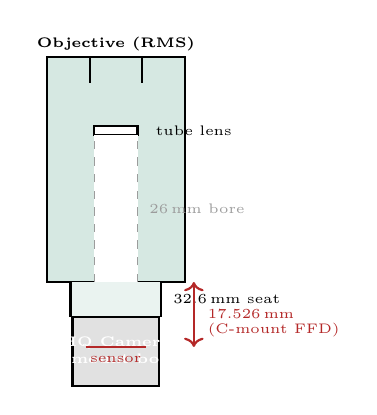
\begin{tikzpicture}[scale=0.55, every node/.style={font=\tiny}]
        % Optics module body (cross-section)
        \fill[unisalzlight] (-1.6, 0) rectangle (1.6, 5.2);
        \draw[thick] (-1.6, 0) rectangle (1.6, 5.2);
        % RMS thread at top
        \draw[thick] (-0.6, 5.2) -- (-0.6, 4.6) (0.6, 5.2) -- (0.6, 4.6);
        \node[align=center] at (0, 5.5) {\textbf{Objective (RMS)}};
        % Tube lens
        \draw[thick, fill=white] (-0.5, 3.4) rectangle (0.5, 3.6);
        \node[right] at (0.7, 3.5) {tube lens};
        % Clear bore
        \fill[white] (-0.5, 0) rectangle (0.5, 3.4);
        \draw[dashed, color=unisalzgray] (-0.5, 0) -- (-0.5, 3.4);
        \draw[dashed, color=unisalzgray] (0.5, 0) -- (0.5, 3.4);
        \node[right, color=unisalzgray] at (0.55, 1.7) {26\,mm bore};
        % C-mount seat
        \fill[unisalzlight!50] (-1.05, -0.8) rectangle (1.05, 0);
        \draw[thick] (-1.05, -0.8) -- (-1.05, 0) -- (-1.6, 0);
        \draw[thick] (1.05, -0.8) -- (1.05, 0) -- (1.6, 0);
        \node[right] at (1.1, -0.4) {32.6\,mm seat};
        % Camera body
        \fill[unisalzgray!30] (-1.0, -2.4) rectangle (1.0, -0.8);
        \draw[thick] (-1.0, -2.4) rectangle (1.0, -0.8);
        \node[align=center, color=white] at (0, -1.6) {\textbf{HQ Camera}\\\textbf{C-mount body}};
        % Sensor plane indicator
        \draw[<->, thick, color=alertred] (1.8, 0) -- (1.8, -1.5);
        \node[right, color=alertred] at (1.9, -0.75) {17.526\,mm};
        \node[right, color=alertred, font=\tiny] at (1.9, -1.1) {(C-mount FFD)};
        % Sensor
        \draw[thick, color=alertred] (-0.7, -1.5) -- (0.7, -1.5);
        \node[below, color=alertred, font=\tiny] at (0, -1.5) {sensor};
      \end{tikzpicture}
    \end{column}
    \begin{column}{0.55\textwidth}
      \small
      \textbf{What changed:}
      \begin{itemize}\itemsep=0pt
        \item \texttt{mount\_height: 4.5 $\to$ 17.526\,mm}
        \item \texttt{sensor\_height: 1 $\to$ 0\,mm}
        \item PCB posts $\to$ smooth flange seat
        \item Cover STL removed (body is its own enclosure)
      \end{itemize}

      \vspace{0.3em}
      \textbf{Geometry:}
      \footnotesize
      \begin{tabular}{@{}lr@{}}
        \toprule
        Flange housing OD (HQ Cam) & 32.0\,mm \\
        Printed seat ID & 32.6\,mm \\
        Slip-fit clearance & 0.3\,mm \\
        Seat depth & 4.0\,mm \\
        Optical clear bore & 26.0\,mm \\
        \bottomrule
      \end{tabular}
    \end{column}
  \end{columns}

\end{frame}

% --------------------------------------------------
% Slide: Why not print a thread
% --------------------------------------------------
\begin{frame}{Design Decision --- Slip-Fit vs.\ Printed Thread}

  \textbf{Why we did not print a 1''-32 UN female C-mount thread.}

  \vspace{0.3em}

  \begin{columns}[T]
    \begin{column}{0.48\textwidth}
      \begin{block}{Printed thread (rejected)}
        \footnotesize
        \begin{itemize}\itemsep=0pt
          \item Pitch 0.794\,mm at 25.4\,mm dia.\ is below FDM tolerance.
          \item Layer adhesion fights the helix; thread strips after a few cycles.
          \item Adds modelling complexity and print time without measurable benefit.
        \end{itemize}
      \end{block}
    \end{column}
    \begin{column}{0.48\textwidth}
      \begin{block}{Slip-fit seat (chosen)}
        \footnotesize
        \begin{itemize}\itemsep=0pt
          \item One smooth bore, robust against print variation.
          \item 0.3\,mm clearance is tighter than typical FDM thread accuracy.
          \item Flange face self-references against printed lip --- gravity does the work in inverted geometry.
          \item Easy to add a printed retainer if needed.
        \end{itemize}
      \end{block}
    \end{column}
  \end{columns}

  \vspace{0.3em}

  \footnotesize
  Both 125\,mm and 150\,mm STLs regenerated automatically: same camera-side
  geometry, different tube length above the seat.

\end{frame}

% --------------------------------------------------
% Slide: Updated stack
% --------------------------------------------------
\begin{frame}{Updated Optical Stack}

  \begin{columns}[T]
    \begin{column}{0.48\textwidth}
      \footnotesize\textbf{Light path (sample $\to$ sensor):}\par
      \vspace{0.3em}
      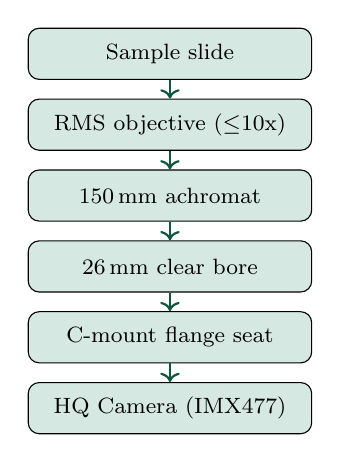
\begin{tikzpicture}[
        box/.style={draw, rounded corners, minimum width=3.6cm, minimum height=0.65cm, align=center, font=\footnotesize, fill=unisalzlight},
        arrow/.style={->, thick, color=unisalz}
      ]
        \node[box] (sample) at (0, 4.5) {Sample slide};
        \node[box] (obj)    at (0, 3.6) {RMS objective ($\leq$10x)};
        \node[box] (tube)   at (0, 2.7) {150\,mm achromat};
        \node[box] (bore)   at (0, 1.8) {26\,mm clear bore};
        \node[box] (seat)   at (0, 0.9) {C-mount flange seat};
        \node[box] (cam)    at (0, 0.0) {HQ Camera (IMX477)};
        \draw[arrow] (sample) -- (obj);
        \draw[arrow] (obj) -- (tube);
        \draw[arrow] (tube) -- (bore);
        \draw[arrow] (bore) -- (seat);
        \draw[arrow] (seat) -- (cam);
      \end{tikzpicture}
    \end{column}
    \begin{column}{0.48\textwidth}
      \small
      \textbf{Output STLs (regenerated):}

      \begin{tabular}{@{}lr@{}}
        \toprule
        File & Size \\
        \midrule
        \texttt{optics\_hq\_150\_rms.stl} & 2.0\,MB \\
        \texttt{optics\_hq\_125\_rms.stl} & 1.9\,MB \\
        \bottomrule
      \end{tabular}

      \vspace{0.5em}
      \textbf{Sensor utilisation:}\\
      150\,mm $\to$ effective FN 19.0\,mm $\to$ \textbf{$\sim$95\,\%} of IMX477 active area.

      \vspace{0.5em}
      \textbf{Build:} \texttt{./build\_optics.sh} regenerates both variants and copies the C-mount override automatically.
    \end{column}
  \end{columns}

\end{frame}

% --------------------------------------------------
% Slide: Roadmap update
% --------------------------------------------------
\begin{frame}{Roadmap Update}

  \footnotesize
  \begin{tabular}{@{}lll@{}}
    \toprule
    \textbf{Phase} & \textbf{Deliverable} & \textbf{Status} \\
    \midrule
    Hardware base       & RPi~5, AI HAT, HQ Cam, OFM server         & \done\ Operational \\
    Parts procurement   & Sangaboard v5, motors, hardware kit       & \done\ Received \\
    Optics design       & Tube lens calc., sensor matching          & \done\ Verified \\
    Custom optics STL   & 125 / 150\,mm + C-mount seat              & \done\ Generated \\
    Tube lens delivery  & Achromatic doublet, 12.7\,mm              & \done\ Received \\
    3D printing         & Body, optics, gears, illumination         & \todo\ Next \\
    ISP tuning file     & IMX477 in OpenFlexure (black-frame fix)   & \wip\ In progress \\
    Mechanical assembly & Microscope build + camera fit             & \todo\ Pending \\
    First light         & Sample on stage, image on web UI          & \todo\ Pending \\
    Stage integration   & Sangaboard wired + \texttt{SangaboardThing}& \todo\ Pending \\
    Time-lapse trial    & 1\,h test run, format $\to$ disk          & \todo\ Pending \\
    Dataset (500--1000) & Annotated frames, CVAT + SAM2             & \todo\ Pending \\
    Model training      & YOLOv8n-seg fine-tune                     & \todo\ Pending \\
    Hailo deployment    & Compiled HEF on NPU                       & \todo\ Pending \\
    \bottomrule
  \end{tabular}

\end{frame}

% --------------------------------------------------
% Slide: What I can add — value beyond the build
% --------------------------------------------------
\begin{frame}{What Else This Project Can Deliver}

  \textbf{Beyond the immediate experiment, the platform produces reusable artifacts.}

  \vspace{0.3em}

  \begin{columns}[T]
    \begin{column}{0.48\textwidth}
      \footnotesize
      \textbf{For the lab:}
      \begin{itemize}\itemsep=0pt
        \item \textbf{Reproducible deploy:} Ansible playbook brings any RPi~5 to "ready" in $<$10\,min.
        \item \textbf{Benchmarked NPU:} Hailo-8 verified at 91.5\,inf/s, 10.9\,ms (YOLOv8s Pose).
        \item \textbf{Dataset pipeline:} CVAT $\to$ SAM2 $\to$ YOLO $\to$ HEF, scriptable end-to-end.
        \item \textbf{Cost ceiling:} entire scope $\sim$300\,EUR; replicable elsewhere.
      \end{itemize}
    \end{column}
    \begin{column}{0.48\textwidth}
      \footnotesize
      \textbf{For the community:}
      \begin{itemize}\itemsep=0pt
        \item \textbf{Upstream contribution:} C-mount seat patch is a candidate PR for OpenFlexure (\texttt{hq\_camera} branch).
        \item \textbf{Pi 5 patches:} pisp tuning, pipewire mask, DKMS ordering --- already filed.
        \item \textbf{Open BOM:} every part referenced by datasheet, no proprietary tooling.
        \item \textbf{HEF zoo:} compiled cell-segmentation model usable on any Hailo-8 device.
      \end{itemize}
    \end{column}
  \end{columns}

\end{frame}

% --------------------------------------------------
% Slide: Value adds — concrete extensions
% --------------------------------------------------
\begin{frame}{Concrete Extensions Worth Discussing}

  \textbf{Each is independently scoped --- pick what fits the timeline.}

  \vspace{0.2em}

  \footnotesize
  \begin{tabular}{@{}p{4.2cm}p{5.5cm}p{2.5cm}@{}}
    \toprule
    \textbf{Extension} & \textbf{Why} & \textbf{Effort} \\
    \midrule
    Incubator-safe enclosure   & 37\,\si{\celsius}/humidity rated; computing stays out & 1--2 weeks \\
    Flat-field calibration     & Removes vignetting + lens shading from raw frames    & 2--3 days \\
    Autofocus via Hailo NPU    & Sharpness inferred online; closes z-loop             & 1 week \\
    Time-lapse scheduler       & Cron + REST; logs to NAS automatically               & 2 days \\
    Live overlay on web UI     & Inference results streamed back to OFM UI            & 1 week \\
    Inverted-stage variant     & Sample on top, objective below --- chip-friendly     & STL fork \\
    Multi-channel illumination & Add fluorescence LEDs (calcein for \ce{Ca^{2+}})     & 2 weeks + parts \\
    \bottomrule
  \end{tabular}

\end{frame}

% --------------------------------------------------
% Slide: Risks remaining
% --------------------------------------------------
\begin{frame}{Risks Still on the Table}

  \footnotesize
  \begin{tabular}{@{}p{3.8cm}p{6.4cm}p{2.2cm}@{}}
    \toprule
    \textbf{Risk} & \textbf{Mitigation} & \textbf{Severity} \\
    \midrule
    Tube lens BFD off datasheet     & \texttt{tube\_lens\_ffd} is one parameter; reprint optics module & Low \\
    Slip-fit too tight or loose     & Adjust seat ID by $\pm$0.1\,mm and rebuild                       & Low \\
    Camera black-frame (ISP tuning) & \texttt{rpicam-still} works; OpenFlexure venv missing pisp tuning file for IMX477 & \alert{Open} \\
    Objective parfocal $\neq$ 45\,mm & 35\,mm variant available; verify before printing                 & Low \\
    Bioreactor flow rate undefined  & Empirical calibration once chip + pump paired                    & Medium \\
    Annotation throughput           & SAM2-assisted; fall back to coarser classes if too slow          & Medium \\
    \bottomrule
  \end{tabular}

\end{frame}

% --------------------------------------------------
% Slide: Immediate next steps
% --------------------------------------------------
\begin{frame}{Immediate Next Steps}

  \textbf{Two-week horizon --- hardware and software in parallel:}

  \vspace{0.3em}

  \footnotesize
  \begin{enumerate}\itemsep=0.15em
    \item \textbf{Print queue:} main body, optics module (150\,mm), gears, condenser, illumination, tools (black PLA / PETG, 0.15\,mm).
    \item \textbf{Verify tube lens BFD.} Check 150\,mm achromat datasheet against \texttt{tube\_lens\_ffd = 146.9\,mm}; adjust and rebuild STL only if different.
    \item \textbf{ISP tuning file.} \texttt{rpicam-still} works; OpenFlexure's \texttt{StreamingPiCamera2} produces black frames --- pisp tuning file for IMX477 is missing in the OpenFlexure venv path. Resolve in parallel with printing.
    \item \textbf{Mechanical assembly.} Insert tube lens, thread objective, slide HQ Camera into C-mount seat.
    \item \textbf{First light.} Mount on dovetail, route ribbon cable, confirm live stream in OpenFlexure web UI.
    \item \textbf{Stage integration.} Wire Sangaboard, flash firmware, switch \texttt{ofm\_config.json} from \texttt{DummyStage} $\to$ \texttt{SangaboardThing}, redeploy via Ansible.
    \item \textbf{Stage calibration.} Step 28BYJ-48 motors, measure step size with calibration slide.
  \end{enumerate}

  \vspace{0.2em}
  \footnotesize After step 7 we are at "first useful image" --- the gate to dataset collection.

\end{frame}

% --------------------------------------------------
% Slide: Geometry — side-window constraint
% --------------------------------------------------
\begin{frame}{Geometry Constraint --- Side Windows Require a Horizontal Axis}

  \begin{columns}[T]
    \begin{column}{0.30\textwidth}
      \centering\footnotesize\textbf{OFM Inverted}\\{\tiny (default)}\par\vspace{0.3em}
      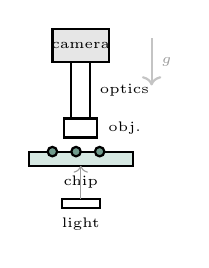
\begin{tikzpicture}[scale=0.60, every node/.style={font=\tiny}]
        \draw[thick,fill=unisalzgray!25] (-0.6,4.0) rectangle (0.6,4.7); \node at (0,4.35) {camera};
        \draw[thick] (-0.2,2.8) rectangle (0.2,4.0); \node[right] at (0.2,3.4) {optics};
        \draw[thick,fill=white] (-0.35,2.4) rectangle (0.35,2.8); \node[right] at (0.38,2.6) {obj.};
        \fill[unisalzlight] (-1.1,1.8) rectangle (1.1,2.1);
        \draw[thick] (-1.1,1.8) rectangle (1.1,2.1); \node[below] at (0,1.8) {chip};
        \foreach \x in {-0.6,-0.1,0.4} { \draw[fill=unisalz!60,thick] (\x,2.1) circle (0.10); }
        \draw[thick,fill=white] (-0.4,0.9) rectangle (0.4,1.1); \node[below] at (0,0.9) {light};
        \draw[->,color=unisalzgray] (0,1.1) -- (0,1.8);
        % gravity arrow
        \draw[->,thick,color=unisalzgray!60] (1.5,4.5) -- (1.5,3.5); \node[right,color=unisalzgray] at (1.5,4.0) {$g$};
      \end{tikzpicture}
      \par\vspace{0.2em}
      {\tiny Optical axis vertical.\\ Bottom window needed.}
    \end{column}
    \begin{column}{0.30\textwidth}
      \centering\footnotesize\textbf{OFM Upright}\par\vspace{0.3em}
      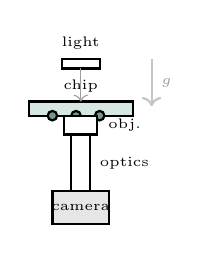
\begin{tikzpicture}[scale=0.60, every node/.style={font=\tiny}]
        \fill[unisalzlight] (-1.1,3.3) rectangle (1.1,3.6);
        \draw[thick] (-1.1,3.3) rectangle (1.1,3.6); \node[above] at (0,3.6) {chip};
        \foreach \x in {-0.6,-0.1,0.4} { \draw[fill=unisalz!60,thick] (\x,3.3) circle (0.10); }
        \draw[thick,fill=white] (-0.35,2.9) rectangle (0.35,3.3); \node[right] at (0.38,3.1) {obj.};
        \draw[thick] (-0.2,1.7) rectangle (0.2,2.9); \node[right] at (0.2,2.3) {optics};
        \draw[thick,fill=unisalzgray!25] (-0.6,1.0) rectangle (0.6,1.7); \node at (0,1.35) {camera};
        \draw[thick,fill=white] (-0.4,4.3) rectangle (0.4,4.5); \node[above] at (0,4.5) {light};
        \draw[->,color=unisalzgray] (0,4.3) -- (0,3.6);
        \draw[->,thick,color=unisalzgray!60] (1.5,4.5) -- (1.5,3.5); \node[right,color=unisalzgray] at (1.5,4.0) {$g$};
      \end{tikzpicture}
      \par\vspace{0.2em}
      {\tiny Optical axis vertical.\\ Top window needed.}
    \end{column}
    \begin{column}{0.36\textwidth}
      \centering\footnotesize\textbf{Required: Horizontal}\par\vspace{0.3em}
      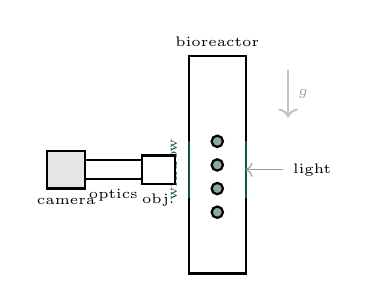
\begin{tikzpicture}[scale=0.60, every node/.style={font=\tiny}]
        % Bioreactor box (upright, side window)
        \draw[thick] (-0.6,0.2) rectangle (0.6,4.8);
        \node[above] at (0,4.8) {bioreactor};
        % Side windows
        \draw[thick,color=unisalz] (-0.6,1.8) -- (-0.6,3.0);
        \draw[thick,color=unisalz] (0.6,1.8) -- (0.6,3.0);
        \node[left,color=unisalz] at (-0.65,2.4) {\rotatebox{90}{window}};
        % cells inside
        \foreach \y in {1.5,2.0,2.5,3.0} {
          \draw[fill=unisalz!50,thick] (0,\y) circle (0.12);
        }
        % Objective approaching from left
        \draw[thick,fill=white] (-1.6,2.1) rectangle (-0.9,2.7);
        \node[below] at (-1.25,2.1) {obj.};
        % Optics tube (horizontal)
        \draw[thick] (-2.8,2.2) rectangle (-1.6,2.6);
        \node[below] at (-2.2,2.2) {optics};
        % Camera (horizontal)
        \draw[thick,fill=unisalzgray!25] (-3.6,2.0) rectangle (-2.8,2.8);
        \node[below] at (-3.2,2.0) {camera};
        % Light from right
        \draw[->,color=unisalzgray] (1.4,2.4) -- (0.6,2.4);
        \node[right] at (1.4,2.4) {light};
        % gravity arrow
        \draw[->,thick,color=unisalzgray!60] (1.5,4.5) -- (1.5,3.5); \node[right,color=unisalzgray] at (1.5,4.0) {$g$};
      \end{tikzpicture}
      \par\vspace{0.2em}
      {\tiny Optical axis horizontal.\\ Gravity $\perp$ optical axis.}
    \end{column}
  \end{columns}

  \vspace{0.2em}
  \footnotesize
  \alert{\textbf{Neither standard OFM orientation works.}}
  Both assume gravity $\parallel$ optical axis; the flexure stage relies on this for preload.
  Rotating 90° puts lateral gravity load on the flexures $\to$ reduced stiffness and drift.
  \textbf{Options:} custom horizontal bracket for OFM $\cdot$ external XYZ stage + camera arm $\cdot$ consult OFM forum.

\end{frame}

% --------------------------------------------------
% Slide: Asks
% --------------------------------------------------
\begin{frame}{What I Need From the Group}

  \small
  \begin{itemize}\itemsep=0.4em
    \item \textbf{Decision:} fluorescence channel from the start, or brightfield first?\\
          \footnotesize (Affects illumination kit. Calcein for \ce{Ca^{2+}} requires 494/517\,nm excitation/emission.)
    \item \textbf{Design input:} the bioreactor's side windows require a horizontal optical axis ---\\
          \footnotesize neither standard OFM orientation works without modification (see previous slide).\\
          \footnotesize \textbf{Key question:} is the chip position fixed, or can a custom mount bring the OFM objective to the window?
    \item \textbf{Input:} mineralization reproducibility is the current open question ---\\
          \footnotesize what are the main variables suspected? (Flow rate? Seeding density? Passage number?)\\
          \footnotesize This drives which parameters to keep fixed in the first imaging protocol.
    \item \textbf{Resource:} access to a compatible chip + perfusion pump for the first wet test.
  \end{itemize}

\end{frame}

% --------------------------------------------------
% Slide: Summary
% --------------------------------------------------
\begin{frame}{Summary}

  \begin{block}{Where we are}
    Hardware fully procured. Custom optics designed and fabricated as STLs.
    First obstacle (camera-side interface) identified and resolved.
  \end{block}

  \begin{block}{What's blocking first light}
    A print run. No \emph{hardware} outstanding.
    Two open software tasks remain: ISP tuning file for the IMX477 (black-frame
    issue in OpenFlexure) and Sangaboard stage integration.
  \end{block}

  \begin{block}{What this platform unlocks}
    Reproducible, low-cost, AI-augmented live-cell imaging. Beyond the hFOB / hMEC experiment, every artifact (STL, ansible role, HEF model) is reusable.
  \end{block}

\end{frame}

% --------------------------------------------------
% Thank you
% --------------------------------------------------
\begin{frame}[plain]
  \centering
  \vfill
  {\Large\color{unisalz} Thank you}

  \vspace{1.0em}
  {\small\color{unisalzgray} Questions, decisions, or new constraints --- now is the cheapest moment to factor them in.\par}

  \vspace{1.5em}

  \begin{tabular}{m{1.0cm}@{\hspace{0.2cm}}l}
    
\includegraphics[height=1.0cm]{img/Siegel-300x300-corpgrey.png} &
    \begin{tabular}{@{}l}
      {\large\color{unisalzgray} universit\"{a}t} \\
      {\large\color{unisalz}\bfseries salzburg}
    \end{tabular}
  \end{tabular}

  \vspace{1.5em}

  \footnotesize
  \href{https://openflexure.org}{openflexure.org} $\cdot$
  \href{https://hailo.ai}{hailo.ai} $\cdot$
  \href{https://github.com/ultralytics/ultralytics}{YOLOv8}
  \vfill
\end{frame}

\end{document}
